\chapter{Gatling - Test Framework}

In diesem Kapitel soll auf das Test Framework \textit{Gatling.io} eingegangen werden. Im Besonderen wird analysiert, was Performance-Tests sind und welche Vorteile diese für den Entwickler bzw. die Softwarearchitektur mit sich bringen.
\newline
Nachdem mögliche Einsatzgebiete von Performance-Tests analysiert wurden, wird auf die \ac{DSL} von Gatling.io eingegangen. Es werden hier die wichtigsten Befehle erläutert.\\
Gatling wurde am 20. Dezember 2011 erstmalig veröffentlicht und ist hauptsächlich in der Programmiersprache Scala implementiert. Laut der Plattform \textit{Open Hub}\footnote{{}Open Hub bietet eine detaillierte Übersicht über Open Source Projekte bzgl. der Aktivitäten, verwendeter Programmiersprachen usw. (vgl. \url{https://www.openhub.net})} hat Gatling über 50k Zeilen an Code bei mehr als 100 Contributors\footnote{{} Als Contributor ist ein Entwickler zu verstehen, der an dem Projekt selbstständig und freiwillig arbeitet.}.\cite{Gatli41:online} Das Tool wurde unter der Apache License 2.0 lizenziert.

\section{Performance-Tests}
\begin{figure}
	{\caption{Software Qualitätseigenschaften}
		\label{fig:ISO9126}}
	{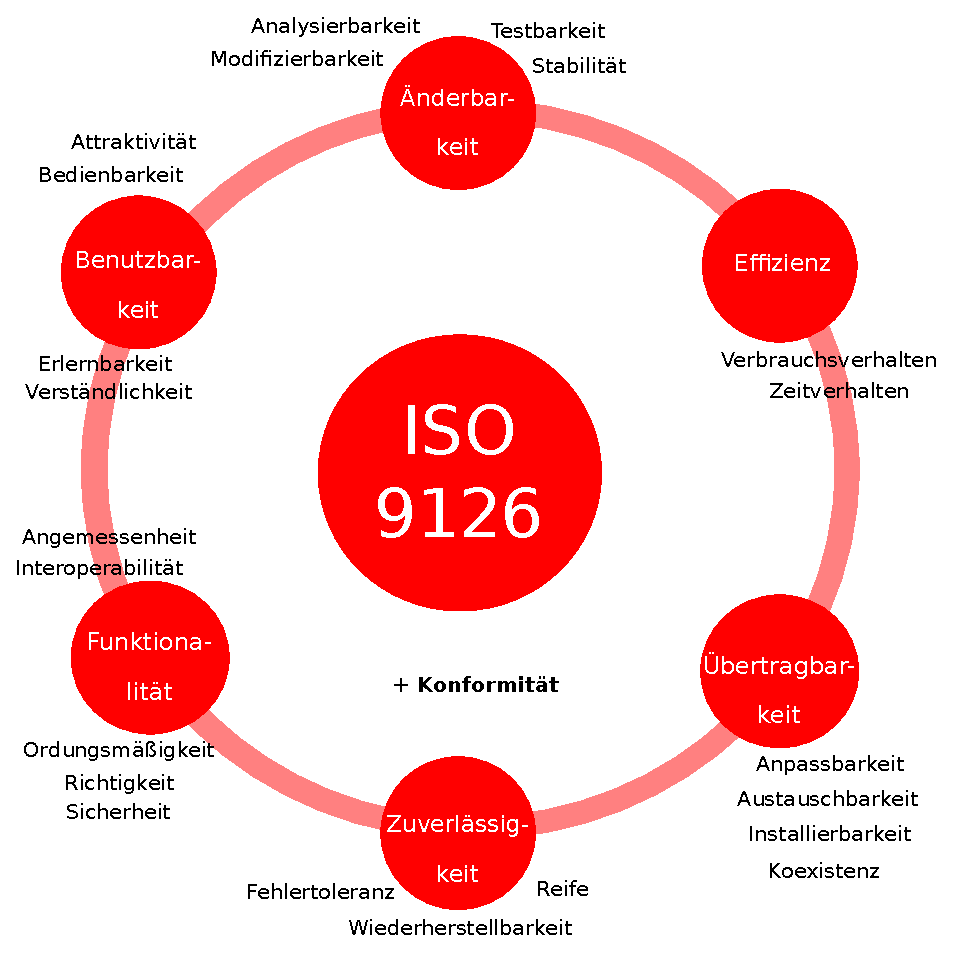
\includegraphics[scale=0.6]{\figdir/ISO9126}}\\
     \tiny{\quelle\url{https://commons.wikimedia.org/w/index.php?curid=52216179}\cite{ISO9126q74:online}}
\end{figure}
In der ISO 9126 wird geregelt wie die Softwarequalität einer Anwendung sichergestellt werden kann.\footnote{{} Die ISO 9126 wurde durch die ISO 25010 abgelöst - äquivalent dazu ist die DIN Norm 66272.}\cite{ISOIEC2533:online} Ein Punkt in der Norm ist \textit{Effizienz}, der in zwei Unterpunkte gegliedert ist:
\begin{itemize}
\item Zeitverhalten
\item und Ressourcenverbrauch.
\end{itemize}
Effizienz beschreibt das Verhältnis zwischen Leistungsniveau der Software und der verwendeten Betriebsmittel. Das Zeitverhalten einer Anwendung beschreibt dabei die Antwort bzw. die Verarbeitungszeit oder auch den Durchsatz bei einer Funktionsausführung. Der Ressourcenverbrauch gibt den Status der verwendeten Betriebsmittel an, wie beispielsweise den verwendeten Speicher, die Netzwerklast bzw. Anzahl Festplattenzugriffe usw.\\
Mit Hilfe von Performance Tests kann das erwartete Zeitverhalten einer Anwendung getestet werden. Durch diese Art der Tests können sogenannte \textit{Bottlenecks} der Anwendung ausfindig gemacht und beseitigt werden. Unter den \textit{Bottlenecks} versteht man einzelne Komponenten der programmierten Anwendung, die den gesamten Worfklow ausbremsen. Als Beispiel könnte folgende Situation dienen:
\begin{itemize}
    \item Eine aufwendigere Berechnung wurde in parallele Tasks ausgelagert
    \item Jeder der Tasks muss eine Datenbankabfrage durchführen, damit die aktuellsten Daten zur Verfügung stehen
    \item Durch diese langwierige Abfrage verzögert sich die gesamte Berechnung
\end{itemize}
Als Bottleneck ist hier die Abfrage zur Datenbank aufzuführen, diese sollte in einen vorgelagerten Prozess abgespalten werden. Auch wenn dieses konstruierte Beispiel sehr einfach und überzogen dargestellt ist, gibt es in echten Anwendungen auch Problembereiche, die vom Entwickler nicht als solche identifiziert werden konnten. Beispielsweise könnte eine Abfrage an eine Schnittstelle unter normalen Bedingungen sofort erledigt sein, unter Last allerdings ändert sich dessen Verhalten. Ohne einen Test, der eine konstruierte Last bzw. Auslastung auf der Anwendung erzeugt, wird diese Art von Fehler nicht entdeckt. Der Administrator kann so vorbeugend im Vornherein die Infrastruktur anpassen, bevor die Anwendung im produktiven Umfeld ist.\newline
 
\subsection{Einsatzgebiete}

Als Einsatzgebiete sind zusammenfassend zu nennen:

\begin{itemize}
    \item Vorhersage von Engpässen (Bottlenecks) in Anwendungen:
   
    Durch einen Test, der eine simulierte Auslastung auf der Anwendung erzeugt, können einzelne Problembereiche der Anwendung aufgezeigt werden.
    
    \item Skalierung der Anwendung:

    Durch Performance-Tests kann eine beliebige Anzahl an Benutzern auf der Anwendung simuliert werden. Es könnte beispielsweise die Skalierung der Anwendung erprobt werden. Hier wird nicht nur die Softwarearchitektur des Programms getestet, sondern auch die IT-Infrastruktur. Durch die genannten Tests könnte beispielsweise aufkommen, dass ein Load-Balancer für eine erwartete Last von 1 Million Benutzern nicht ausreichend ist.
    
    \item Feedback für Benutzer verbessern:
    
    Der Benutzer der Anwendung bekommt ein besseres Produkt mit schnelleren Antwortzeiten, was insgesamt die Zufriedenheit beim Kunden / Benutzer verbessert.    
    
    \item Verbesserung / Optimierung der Software Architektur:
    
    Durch Erfahrungswerte aus vorhergehenden Tests kann langfristig die Softwarearchitektur angepasst bzw. verändert werden. Die Anwendung kann skalierbarer entworfen und geplant werden. Auch das Programmierverhalten der Entwickler wird dadurch positiv beeinflusst. Durch Erfahrungswerte können Fehler schon während der Entwicklungszeit aufgedeckt und verhindert werden. So werden Optimierungen während der Entwicklungsphase durchgeführt. 

\end{itemize}

\subsection{Herausforderungen bei Performance Tests}

Wichtig bei Performance Tests bzw. generell ist die genaue Definition eines zu erreichenden Ziels. Was genau soll als Ergebnis des Tests herausgefunden werden? Nur so kann die Testumgebung dementsprechend geplant und durchgeführt werden.\footnote{In der Praxis wird der Begriff \glqq Performance Test\grqq{} äquivalent für Stress Tests bzw. Last Tests verwendet.\cite{Lasttest51:online}}\\
Performance Tests sind abhängig von der zu erwarteten Leistung. Sicherlich ist es nicht sinnvoll als \glqq kleines\grqq{} Startup mit einer Million von Requests zu rechnen. Die Verhältnisse von eingesetzter Architektur bzw. Betriebsmitteln zu der erwarteten Nutzungsintensität muss gegeben sein. Bei einem Performance Tests wird zwangsläufig irgendwann der Punkt kommen an dem die Anwendung ein deutlich verlangsamtes Ansprechverhalten zeigt. Diesen Punkt muss jeder Software Ingenieur bzw. Manager individuell für das eigene Produkt passend wählen.\\
Es ist darauf zu achten, dass die Testbedingungen möglichst realistisch und ähnlich zu der Produktivumgebung zu wählen sind. So muss beispielsweise beim Testen einer Anwendung auch berücksichtigt werden, dass es zu Verbindungsabbrüchen, unterschiedlichen Nutzungsarten, verschiedene Clients und dergleichen kommen kann. Um möglichst viele Szenarien testen zu können muss im Vorfeld eine Analyse durchgeführt werden, wie die Anwendung hauptsächlich benutzt werden wird. So können Parameter wie die erwartete Benutzerzahl, verwendete Client Konfigurationen usw. herausgefunden und getestet werden.

\section{Gatling - Features}

%https://gatling.io/docs/current/cheat-sheet/

\subsection{Gatling DSL}

\begin{table}[]
\centering
\caption{Cheat-Sheet DSL Gatling.io}
\label{table_cheatSheetDSL}
\begin{tabular}{|
>{\columncolor[HTML]{FCFF2F}}l |
>{\columncolor[HTML]{67FD9A}}l |}
\hline
\cellcolor[HTML]{C0C0C0}Befehl & \cellcolor[HTML]{C0C0C0}Funktionsweise \\ \hline
{\color[HTML]{333333} Erster Test} & Testfunktion \\ \hline
Test & Testfunktion \\ \hline
\end{tabular}

\end{table}
%Tabelle mit wichtigsten Befehlen zeigen


\subsection{Metriken}

Gatling.io sammelt nach erfolgreichem Testen einer Anwendung die gemessenen Metriken in einem Bericht und stellt diese dem Benutzer zur Verfügung. In Abbildung \ref{fig:gatlingMetriken} ist exemplarisch ein Bericht aufgezeigt. In der Übersicht ist in einem Säulendiagramm das Antwortverhalten gegliedert, bspw. grüner Balken hat eine Antwortzeit von unter 800 ms. Außerdem lässt sich erkennen wie viele Requests insgesamt durchgeführt wurden, wie viele fehlgeschlagen sind, sowie die erfolgreich beantworteten Requests.
\begin{figure}
	{\caption{Gatling Metriken}
		\label{fig:gatlingMetriken}}
	{\includegraphics[scale=0.3]{\figdir/gatlingMetriken}}\\
	\tiny{\quelle\url{https://gatling.io/wp-content/uploads/2016/12/rapport.png}}
\end{figure}



\section{Continous Integration}

\begin{figure}
	{\caption{Continous Integration Prozess}
		\label{fig:continousIntegration}}
	{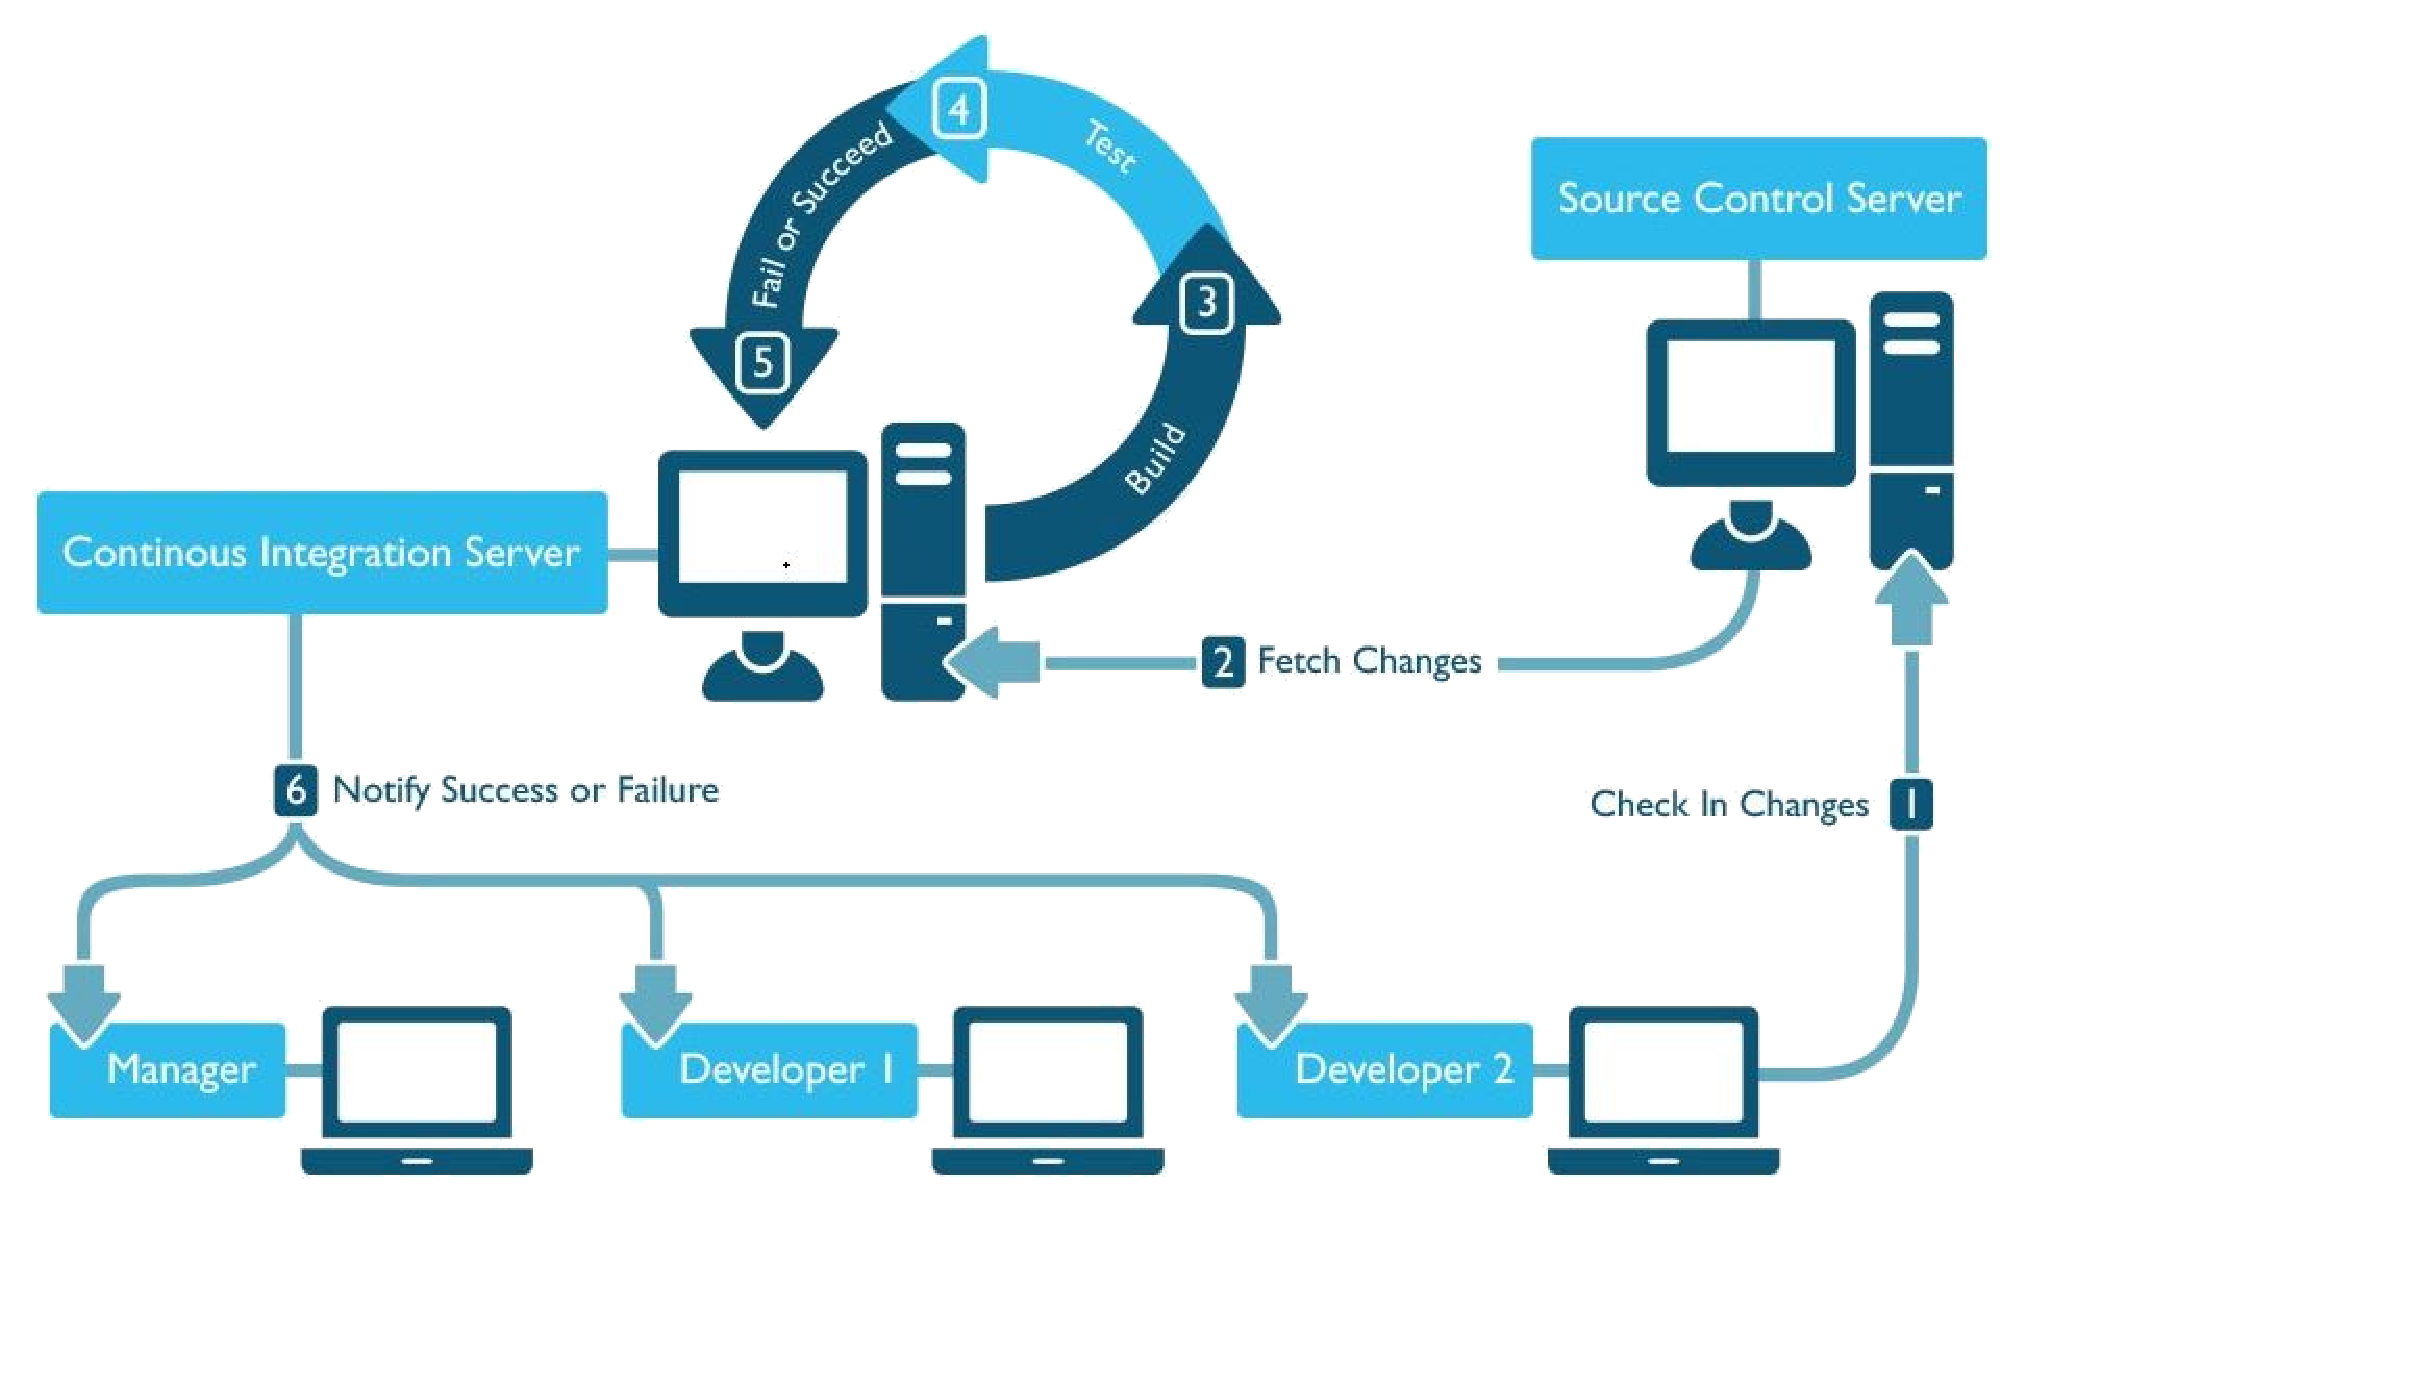
\includegraphics[scale=0.5]{\figdir/CI}}
	\tiny{\quelle\url{http://www.anarsolutions.com/making-ci-effective-size-organization/}}
\end{figure}

Der Einsatz von Buildservern in einer Continous Integration Umgebung gehört mittlerweile zu den Standard Werkzeugen eines Entwicklerteams. Aber was ist Continous Integration und wie können Lasttests in diesen Prozess eingebunden werden?\\
In Abbildung \ref{fig:continousIntegration} ist ein typischer Continous Integration Prozess dargestellt. Die Entwickler pushen ihren modifizierten Sourcecode in den Source Control Server. Dieser kann ein GIT Repository oder ein ähnliches Tool wie \ac{TFS} der Firma Microsoft sein. Dann kommt der eigentliche Buildserver ins Spiel. Dieser holt die vorgenommen Änderungen vom Source Control Server und versucht das Projekt zu kompilieren. Anschließend werden die definierten Tests ausgeführt und sowohl im Erfolgs- als auch im Fehlerfall die Entwickler bzw. Teamleiter informiert. Die Meldung dass der Vorgang erfolgreich durchgeführt wurde, wird langfristig wahrscheinlich überflüssig. Als Mittelweg wäre empfehlenswert, dass nach einem fehlgeschlagenen Versuch der erstmalige erfolgreiche Vorgang als Erfolgsmeldung übermittelt wird. Durch diesen Prozess bekommen die Entwickler schnelles Feedback in Fehlerfällen und können diese beheben.\\
Abbildung \ref{fig:jenkinsBuildResult} zeigt einen Graphen, der auf dem Buildserver \glqq Jenkins\grqq{} während eines Buildvorgangs generiert wurde. Die Grafik zeigt den \glqq Performance Trend\grqq{} einer Anwendung über mehrere Analysen hinweg. Wie aus dem Graph entnommen werden kann, gab es zwischen dem achten und zehnten Buildvorgang stetige Performance Probleme, die aber dann im elften Buildvorgang gelöst werden konnten. So wurden potentielle Bottlenecks, die unabsichtlich durch den Entwickler eingebaut wurden entdeckt und konnten nach dem Buildvorgang behoben werden. Die Anwendung war nicht im Produktivbetrieb, als diese Fehler entdeckt und behoben wurden. Diese Tatsache zeigt den klaren Vorteil von Performance Tests in einem Continous Integration Prozess auf, da die Fehler automatisch noch vor dem Release der Software entdeckt und behoben werden können.
\begin{figure}
	{\caption{Ergebnis der Analyse am Jenkins Buildserver}
		\label{fig:jenkinsBuildResult}}
	{\includegraphics[scale=0.3]{\figdir/jenkinsResult}}\\~\\
				\tiny{\quelle\url{https://gatling.io/wp-content/uploads/2016/12/jenkins2.png}}
\end{figure}


\section{Anwendungsfall - Performance Test mit Gatling}
In diesem Unterkapitel soll auf den grundsätzlichen Aufbau eines Gatling Tests eingangen werden.\\
Gatling Tests sind in der Programmiersprache Scala\footnote{{} Scala ist eine Java-ähnliche Sprache, die auf der \ac{JVM} läuft.} implementiert.
Im Code-Beispiel \ref{testCodingSample} ist beispielhaft ein solcher Test dargestellt. Dieser soll die Schnittstelle für das zufällige Abholen eines Witzes auf Last testen. Die grundsätzliche Funktionsweise der Schnittstelle wird an dieser Stelle vorausgesetzt. Dies muss im Vornherein durch Unit - bzw. Integrationstests sichergestellt werden. Für das Testen der Auslastung müssen allerdings einige Details über die Schnittstelle bekannt sein. So muss u.a. der Server mit zugehörigem Port, sowie der genaue Aufbau der Schnittstelle für den Entwickler einsehbar sein. Dieser Aspekt wird an dieser Stelle erwähnt, da es in größeren Unternehmen durchaus sein könnte, dass unabhängige Teams die gleiche Anwendung testen müssen. In diesem Fall hätte der Entwickler des Performance-Tests, nur die Black-Box-Sicht auf die bereits programmierte Anwendung. Das Code Beispiel \ref{testCodingSample} soll nun im Detail erläutert werden.\\
Zuerst werden die notwendigen Bibliotheken über \glqq Import-Befehle\grqq{} geladen. Die Klasse \glqq RandomJokeSimulation\grqq{} erbt von der definierten Klasse \glqq Simulation\grqq{}.\footnote{{} Jeder Gatling.io Test muss von der Simulation Klasse erben.} Anschließend wird die Verbindung konfiguriert, sowie der notwendige Test-Request zusammengebaut. In diesem Beispiel läuft die Anwendung im internen Netz an der Adresse \glqq http://192.168.111.20\grqq{} auf Port 58080. Damit der Request vom Server akzeptiert wird, werden die notwendigen Header gesetzt.\\
Anschließend wird die zu testende Logik, in Gatling.io \glqq Scenario\grqq{} genannt, implementiert. Das Scenario bekommt einen Namen zugewiesen und die Aufforderung, wie oft dieses ausgeführt werden soll. Zudem wird der genaue Pfad der Schnittstelle definiert und die \ac{HTTP} Methode, die auf die \ac{REST} Schnittstelle ausgeführt werden soll, ausgewählt.\\
Der Lasttest soll möglichst unter den Bedingungen durchgeführt werden, die auch im produktiven System aktiv sind. So ist es unrealistisch anzunehmen dass 1000 Benutzer exakt zeitgleich die Abfrage auf die Schnittstelle absetzen. Es ist vielmehr anzunehmen, dass die Benutzeranzahl mit zunehmender Laufzeit des Programms ansteigen wird. Genau diese Funktionalität bietet Gatling.io an. Zur Test Laufzeit können kontinuierlich, dies ist konfigurierbar, neue Benutzer erstellt werden, die auch Abfragen auf die Schnittstelle absetzen. So kann ein realistischer Use-Case getestet werden.\\ 

\begin{minipage}{\linewidth}
\begin{lstlisting}[frame=single,caption=Testabfrage auf Schnittstelle in Gatling, label=testCodingSample, language=Scala]
import io.gatling.core.Predef._
import io.gatling.http.Predef._
import scala.concurrent.duration._

class RandomJokeSimulation extends Simulation {
    val httpConf = http
        .baseURL("http://192.168.111.20:58080")
        .acceptHeader("application/json")
        .acceptEncodingHeader("gzip, deflate")
        .userAgentHeader("Mozilla/5.0 (Windows NT 5.1; rv:31.0) Gecko/20100101 Firefox/31.0")

    val scn = scenario("RandomJokeSimulation").repeat(100) {
        exec(http("getRandomJoke")
        .get("/api/v1/joke/random"))
    }    

    setUp(
        scn.inject(atOnceUsers(100))
    ).protocols(httpConf)
}
\end{lstlisting}
\end{minipage}
Als Alternative zu Gatling.io ist \textit{Apache JMeter} zu nennen.\footnote{{} vgl. \url{https://jmeter.apache.org/}} JMeter wurde im Jahr 1998 erstmalig veröffentlicht und wurde hauptsächlich in Java implementiert.\footnote{{} Der direkte Vergleich von JMeter zu Gatling ist hier aufgezeigt.\cite{JMetervs63:online}}

\section{Zwischenfazit Lasttests}

Performance- oder Lasttests sind notwendig um eine stabile Anwendung bzw. API zu entwickeln.
Langfristig wird sich die Architektur bzw. der Programmierprozess verbessern, wenn die Ergebnisse der Tests analysiert, ausgewertet und auch für zukünftige Entwicklungen berücksichtigt werden. Durch die Integration in eine Continuous Integration Umgebung wird ein schnelles Feedback der Tests an die Entwickler garantiert und diese können noch während der Entwicklungsphase aufkommende negative Trends bzgl. der Antwortzeiten / Performance der Anwendung analysieren und beheben. So wird garantiert, dass eine umfangreich getestete Software keine bösen Überraschungen bei aufkommender Last zeigt. Mit Gatling wird ein umfangreiches Performance Test Tool angeboten, das sowohl eine gute Integration in einen Buildserver, wie beispielsweise Jenkins bietet, als auch mit einer \ac{GUI} einfach Operationen durchführen lässt.


